\documentclass[pdflatex,11pt]{aghdpl}
% \documentclass{aghdpl}               % przy kompilacji programem latex
% \documentclass[pdflatex,en]{aghdpl}  % praca w j?zyku angielskim
\usepackage[polish]{babel}
\usepackage[utf8]{inputenc}

% dodatkowe pakiety
\usepackage{enumerate}
\usepackage{listings}
\lstloadlanguages{TeX}



%---------------------------------------------------------------------------

\author{Dorota Wojtałow, Jacek Złydach}
\shortauthor{D. Wojtałów, J. Złydach}
%\shortauthor{M. Szpyrka}

\titlePL{Symulacja rozprzestrzeniania się dymu i ognia w oparciu o niehomogeniczne automaty komórkowe}
\titleEN{Simulation of fire and smoke by using non-homogeous cellular automata}
%\titleEN{Thesis in \LaTeX}


\thesistypePL{Praca inżynierska}

\supervisorPL{dr inż. Jarosław Wąs}
\supervisorEN{Jarosław Wąs Ph.D}

\date{2010}

\facultyPL{Wydział Elektrotechniki, Automatyki, Informatyki i Elektroniki}

\acknowledgements{Serdecznie dziękujemy \dots }

%---------------------------------------------------------------------------

\begin{document}

\titlepages

\tableofcontents
\clearpage

\chapter{Wstęp}
\label{cha:wstep}
%TODO refactoring - czemu nie potrafie zrobić pustej linii przed tezą?!?!?!

%wg. strong Wojnickiego 5 pktow które powinny znaleźć się we wstępie:
% 1. Co - przediot, problem pracy
% 2. Jak - metoda, krotko
% 3. Dlaczego - źrodla problemu badawczego
% 4. Po co - implikacje, konsekwencje, walory
% 5. Co w kolejnych rozdziałach
\section{Temat pracy} % 1 Co

Tematem pracy jest stworzenie symulacji rozprzestrzeniania się dymu i ognia 
w opraciu o niehomogeniczne automaty komórkowe. Zakres pracy obejmuje stworzenie symulacji rozchodzenia się dymu i ognia na podstawie automatów komórkowych wraz z jej wizualizacją, a także walidację stworzonego modelu. 
Celem pracy jest pokazanie możliwości niehomogenicznych automatów komórkowych jako narzędzia umożliwiającego 
odzwierciedlenie rzeczywistego rozprzestrzeniania się dymu i ognia podczas pożaru. 

\section {Geneza tematu} %3 i 4 - Dlaczego i po co

W dobie wszechobecnej urbanizacji i ciągłego budownictwa, wraz ze wzrostem świadomości dotyczącej bezpieczeństwa
pożarowego oraz zaangażowania w jego zagwarantowaniu pojawiła się potrzeba możliwości modelowania i obserwacji rozprzestrzeniania się ognia w zamkniętych budynkach.
Wspomniane symulacje pożarów wykazują szereg zastosowań. Są z powodzeniem wykorzystywane w śledztwach. Dają możliwość odtworzenia przebiegu zdarzeń i porównania z wynikami oględzin. Umożliwiają
zbadanie prototypu budynku pod kątem gwarancji bezpieczeństwa pożarowego. 
Ułatwiają projektowanie systemów oddymiania. W połączeniu z modelami ewakuacji ludzi
stanowią kompleksowy system ułatwiający tworzenie bezpiecznych budowli.

W ostatnich latach powstał szereg programów umożliwiających wizualizcję symulacji rozchodzenia ognia. Opracowane dotychczas rozwiązania swoje działanie 
opierają na metodach numerycznej dynamiki płynów (ang. Computational Fluid Dynamics). Niewątpliwą zaletą numerycznego podejścia jest dokładność wyników. 
Głównymi wadami jest złożoność obliczeń i stopień komplikacji modelu. 
Niehomogeniczne automaty komórkowe umożliwiają znaczne uproszczenie modelu. Uproszczenie modelu powoduje z kolei redukcję złożoności
obliczeń czyniąc automaty komórkowe szczególnie dogodną metodą w przypadku tworzenia prototypów oraz symulacji czasu rzeczywistego.

%dopisać coś jeszcze o tym, że nie ma takich symulatorów wyk. automaty komórkowe 



\textbf{Teza} Wykorzystując zasady tworzenia automatów komórkowych oraz w oparciu o prawa fizyki można w realistyczny sposób
przy użyciu niehomogenicznych 
automatów komórkowych
zamodelować zjawiska rozchodzenia się ognia i dymu podczas pożaru.

W celu wykazania powyższej tezy przeprowadzono następujące działania:
\begin{itemize}
\item Przeprowadzono badania dotyczące zjawisk fizycznych zachodzących podczas pożaru.
\item Zidentyfikowano czynniki mające kluczowy wpływ na kształt i charakter pożaru.
\item Zaproponowano model niehomogenicznego automatu komórkowego odzwierciedlającego prawa fizyczne.
\item Zaimplementowano opracowany algorytm wraz z wizualizacją wyników oraz możliwością edycji danych wejściowych oraz kontroli symulacji w czasie rzeczywistym.
\item Dokonano weryfikacji jakościowej zaproponowanego modelu.
\end{itemize}

\section {Realizacja projektu} % 2 - jak
Praca została zrealizowana jako wolnostojąca aplikacja komputerowa napisana w języku Java. Do renderowania grafiki trójwymiarowej
zostala użyta biblioteka graficzna Java3D. Aplikacja została przetestowana z wykorzystaniem biblioteki JUnit4. 

\section{Zawartość pracy} % 5 - co w kolejnych rozdziałach Tutaj na pewno trzeba dać odnośniki do rozdziałów a nie tytuły!
Praca składa się z [iluś] rozdziałów. 
W pierwszym rozdziale znajdują się podstawy teoretyczne, związane zarówno z modelowanymi zjawiskami fizycznymi jak i użytym algorytmem.
Rozdział Modele symulacji zawiera propozycje zweryfikowanych modeli rozprzestrzeniania się dymu i ognia zaprojektowanych w oparciu
o niehomogeniczne automaty komórkowe. Rozdział Implementacja przedstawia sposób realizacji projektu, napotkane problemy oraz 
ich rozwiązania. Opisuje możliwości graficznego interfejsu użytkownika oraz sposób korzystania z niego.
 % W podsumowaniu znajduje się podsumowanie.... nie wiem jeszcze jak to ładnie ująć
%cos wiecej o rozdzialach. dopisac jak będa gotowe

\chapter {Projekt}
\label{cha:projekt}
\section {Główne zalożenia}
\begin {itemize}
\item Głównym celem projektu jest stworzenie i weryfikacja modelu rozprzestrzeniania się ognia wykorzystując niehomogeniczne automaty
komórkowe. Nacisk z pracy został położony na opracowanie algorytmu najdokładniej oddającego rzeczywistość.
\item Projekt obejmuje także swtworzenie uproszczonej wizualizacji symulacji oraz graficznego interfejsu użytkownika (GUI).
\item Interfejs aplikacji powinien umożliwiać edycję budynku w którym przeprowadzana jest symulacja: dodawanie elementów konstrukcji, 
określanie materiałów z których zostały stworzone. 
\item Użytkownik powinien mieć możliwość określenia źródła ognia: zarówno jego miejsca jak i temperatury początkowej.
\item Aplikacja powinna umożliwiać także kontrolę nad symulacją: możliwość zatrzymania symulacji, wznowienia, rozpoczęcia od początku,
a także dostosowanie tempa symulacji umożliwiającego obserwację zjawisk fizycznych.
\end {itemize}
\section {Architektura aplikacji}
% w bibliografi powinno byc coś o tej architekturze i def. aktywnego modelu
Aplikacja została zaprojektowana zgodnie z architekturą Model-View-Controller.
Poniższy schemat przedstawia typowy przykład architektury Model-View-Controller:
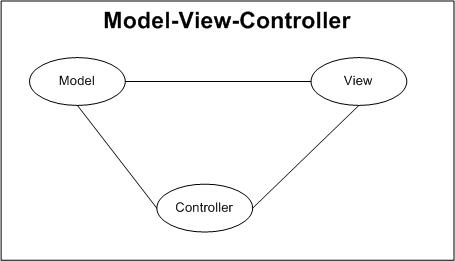
\includegraphics{MVC.jpeg}
W omawianej pracy została zaimplementowana pewna odmiana typowej architektury Model-Widok-Kontroler.
Najodpowiedniej przedstawia ją poniższy rysunek:
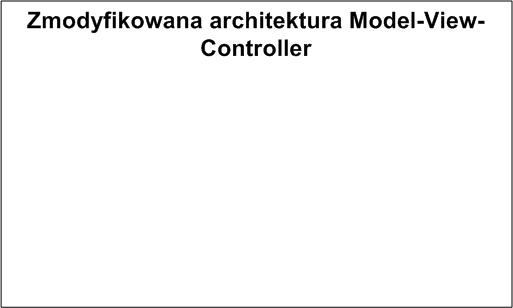
\includegraphics{modifiedMVC.jpeg}
Kontroler odpowiada za pobranie danych od użytkownika, ich przetworzenie oraz dostarczenie do modelu.
Został zastosowany przypadek aktywnego modelu, który zgodnie z definicją potrafi zmieniać swój stan 
bez względu na akcje wykonywane przez użytkownika. W projekcie symulacji pożaru aktywność modelu polega na 
wykonywaniu pętli symulacji, związanych z nią obliczeń, powiadamianiu widoku o zachodzących zmianach oraz
końcu symulacji. Widok odpowiada jedynie za prezentację wyników symulacji.
Wybrana architektura umożliwia elastyczny rozwój aplikacji. Wprowadzony podział na trzy odrębne moduły pozwala
na nieograniczone zmiany w każdym z nich, nie powodując konieczności zmian innych części aplikacji.
Inną zaletą separacji jest łatwość testowania poszcególnych modułów osobno. 
\section {Moduły}
\section {Obiekty}

% itd.
% \appendix
% \include{dodatekA}
% \include{dodatekB}
% itd.

\bibliography{bibliografia}

\end{document}

